\documentclass[12pt,a4paper]{article}
\usepackage[utf8]{inputenc}
\usepackage[margin=0.65in]{geometry}
\usepackage{graphicx}
\usepackage{booktabs}
\usepackage{array}
\usepackage{hyperref}
\usepackage{xcolor}
\usepackage{tikz}
\usepackage{enumitem}
\usepackage{float}
\usepackage{multicol}

\usetikzlibrary{shapes,arrows,positioning,shapes.geometric,arrows.meta,shadows,calc}

% Balanced spacing
\setlength{\parskip}{0.4em}
\setlength{\tabcolsep}{5pt}
\renewcommand{\arraystretch}{1.0}
\setlist{nosep, leftmargin=*}

% Remove headers/footers
\pagestyle{empty}

% Colors
\definecolor{isroblue}{RGB}{0, 51, 102}
\definecolor{perceptblue}{RGB}{52, 152, 219}
\definecolor{memoryviolet}{RGB}{142, 68, 173}
\definecolor{reasonorange}{RGB}{230, 126, 34}
\definecolor{actiongreen}{RGB}{39, 174, 96}
\definecolor{learnlime}{RGB}{241, 196, 15}
\definecolor{llmred}{RGB}{192, 57, 43}
\definecolor{envgray}{RGB}{149, 165, 166}
\hypersetup{colorlinks=true,linkcolor=isroblue,urlcolor=isroblue}

% Section spacing
\usepackage{titlesec}
\titlespacing*{\section}{0pt}{2.5ex}{1.2ex}
\titlespacing*{\subsection}{0pt}{1.8ex}{0.8ex}

\title{
    \vspace{-2cm}
    \textbf{CS6312E: Intelligent Agents - Design Document}\\
    \large Generative Agents for Realistic Social Simulation\\
    \normalsize Capstone Project 2025-2026
}
\author{
    Yashvardhan (M250570CS) \quad Prakash Kumar Sarangi (M251250CS)
}
\date{January 28, 2026}

\begin{document}

\maketitle
\vspace{-0.8cm}

%----------------------------------------------------------
\section{PEAS Analysis}
%----------------------------------------------------------

\subsection{Performance Measures}

\begin{table}[H]
\centering
\small
\begin{tabular}{|l|l|l|}
\hline
\textbf{Metric} & \textbf{Description} & \textbf{Measurement} \\
\hline
Goal Completion & Successfully completing daily tasks & \% of planned tasks completed \\
Social Engagement & Quality of interactions with others & Conversations per day \\
Emotional Stability & Maintaining balanced emotional state & Variance in mood scores \\
Relationship Building & Forming social connections & Relationship strength (0-100) \\
Survival Contribution & Contributing to base operations & Task contribution score \\
\hline
\end{tabular}
\end{table}

\subsection{Environment Description}
\textbf{Setting:} Aryabhata Station is ISRO's first permanent lunar base, located at the Moon's South Pole (Year 2035). It has 8 interconnected modules: Mission Control, Agri Lab, Mess Hall, Rec Room, Crew Quarters, Medical Bay, Comms Tower, and Mining Tunnel.

\subsection{Actuators (Actions)}

\begin{table}[H]
\centering
\small
\begin{tabular}{|l|l|l|}
\hline
\textbf{Actuator} & \textbf{Function} & \textbf{Parameters} \\
\hline
\texttt{move(location)} & Navigate to a location & Target location ID \\
\texttt{talk(agent, message)} & Communicate with agent & Target agent, message \\
\texttt{work(task)} & Perform work activity & Task type, duration \\
\texttt{rest()} & Take rest/sleep & Duration \\
\texttt{observe()} & Actively scan environment & Observation radius \\
\texttt{interact(object)} & Use equipment/objects & Object ID \\
\hline
\end{tabular}
\end{table}

\subsection{Sensors (Perceptions)}

\begin{table}[H]
\centering
\small
\begin{tabular}{|l|l|l|}
\hline
\textbf{Sensor} & \textbf{Input Type} & \textbf{Range} \\
\hline
\texttt{see\_agents()} & Detect nearby agents & Current location \\
\texttt{hear\_conversations()} & Overhear dialogue & Adjacent locations \\
\texttt{check\_time()} & Current simulation time & Global \\
\texttt{observe\_events()} & Detect environmental events & Current location \\
\texttt{check\_status()} & Self-status (energy, mood) & Internal \\
\texttt{read\_messages()} & Check communications & Personal queue \\
\hline
\end{tabular}
\end{table}


%----------------------------------------------------------
\section{Environment Properties}
%----------------------------------------------------------

\begin{table}[H]
\centering
\small
\begin{tabular}{|l|l|p{7cm}|}
\hline
\textbf{Property} & \textbf{Classification} & \textbf{Justification} \\
\hline
Observable & Partially Observable & Agents perceive only current and adjacent locations \\
Determinism & Stochastic & Other agents' responses unpredictable; random events occur \\
Episodic/Sequential & Sequential & Past interactions influence future behaviors \\
Static/Dynamic & Dynamic & Environment changes continuously as agents act \\
Discrete/Continuous & Discrete & Time in fixed steps; locations are discrete nodes \\
Agent Type & Multi-agent & 8 agents interact (cooperative + competitive) \\
\hline
\end{tabular}
\end{table}

%----------------------------------------------------------
\section{Architecture Choice}
%----------------------------------------------------------

\subsection{Selected Architecture: Hybrid Goal-Based + Utility-Based Agent}

Our design uses a hybrid architecture that combines \textbf{Goal-Based} components (where explicit objectives drive planning) with \textbf{Utility-Based} components (for weighing importance of competing goals). We chose this because pure architectures have limitations: simple reflex agents can't handle memory, model-based approaches lack goal-direction, pure goal-based can't prioritize well, and pure utility-based is computationally expensive.

\subsection{Component Justification}

\begin{table}[H]
\centering
\small
\begin{tabular}{|l|l|p{6cm}|}
\hline
\textbf{Component} & \textbf{Architecture Type} & \textbf{Reason} \\
\hline
Daily Planning & Goal-Based & Explicit objectives guide behavior \\
Action Selection & Utility-Based & Weighs competing priorities \\
Memory Retrieval & Utility-Based & Scores by recency, importance, relevance \\
Social Behavior & Goal-Based & Relationship maintenance as goals \\
\hline
\end{tabular}
\end{table}

\subsection{Architecture Diagram}

\begin{center}
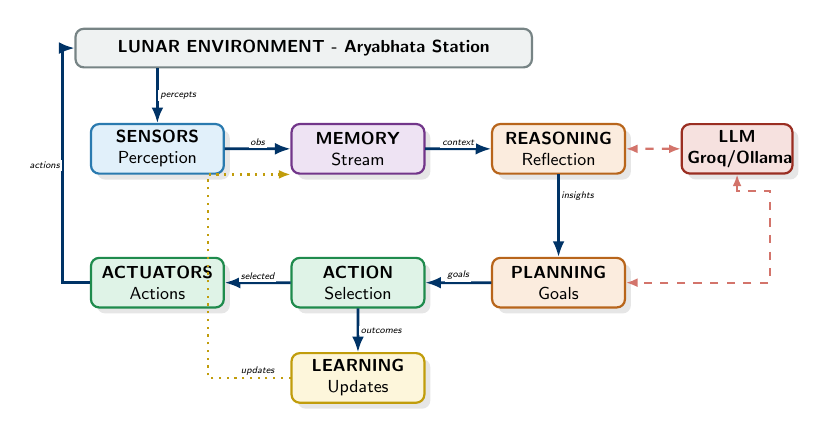
\begin{tikzpicture}[
    scale=0.70, transform shape,
    node distance=0.9cm and 1.2cm,
    auto,
    block/.style={
        rectangle, draw=#1!80!black, thick, fill=#1!15, 
        text width=2.2cm, inner sep=3pt, align=center, 
        minimum height=0.9cm, rounded corners=3pt, 
        drop shadow={opacity=0.2}, font=\small\sffamily
    },
    envblock/.style={
        rectangle, draw=envgray!80!black, thick, fill=envgray!15, 
        text width=8cm, inner sep=4pt, align=center, 
        minimum height=0.7cm, rounded corners=3pt, font=\small\sffamily\bfseries
    },
    llmblock/.style={
        rectangle, draw=llmred!80!black, thick, fill=llmred!15, 
        text width=1.8cm, inner sep=3pt, align=center, 
        minimum height=0.8cm, rounded corners=3pt, 
        drop shadow={opacity=0.2}, font=\small\sffamily\bfseries
    },
    mainflow/.style={draw=isroblue, line width=1pt, -{Latex[length=2mm, width=1.5mm]}},
    llmflow/.style={draw=llmred!70, line width=0.8pt, dashed, {Latex[length=1.5mm]}-{Latex[length=1.5mm]}},
    learnflow/.style={draw=learnlime!80!black, line width=0.8pt, dotted, -{Latex[length=1.5mm]}},
    flowlabel/.style={font=\tiny\sffamily\itshape, fill=white, inner sep=1pt}
]
    \node[envblock] (env) {LUNAR ENVIRONMENT - Aryabhata Station};
    \node[block=perceptblue, below=1cm of env.south west, anchor=north, xshift=1.5cm] (sensors) {\textbf{SENSORS}\\Perception};
    \node[block=memoryviolet, right=of sensors] (memory) {\textbf{MEMORY}\\Stream};
    \node[block=reasonorange, right=of memory] (reasoning) {\textbf{REASONING}\\Reflection};
    \node[llmblock, right=1cm of reasoning] (llm) {LLM\\Groq/Ollama};
    \node[block=actiongreen, below=1.5cm of sensors] (actuators) {\textbf{ACTUATORS}\\Actions};
    \node[block=actiongreen, right=of actuators] (action) {\textbf{ACTION}\\Selection};
    \node[block=reasonorange, right=of action] (planning) {\textbf{PLANNING}\\Goals};
    \node[block=learnlime, below=0.8cm of action] (learning) {\textbf{LEARNING}\\Updates};

    \draw[mainflow] (env.south -| sensors) -- node[flowlabel, right] {percepts} (sensors.north);
    \draw[mainflow] (sensors) -- node[flowlabel, above] {obs} (memory);
    \draw[mainflow] (memory) -- node[flowlabel, above] {context} (reasoning);
    \draw[mainflow] (reasoning.south) -- ++(0,-0.4) -| node[flowlabel, pos=0.25, right] {insights} (planning.north);
    \draw[mainflow] (planning) -- node[flowlabel, above] {goals} (action);
    \draw[mainflow] (action) -- node[flowlabel, above] {selected} (actuators);
    \draw[mainflow] (actuators.west) -- ++(-0.5,0) |- node[flowlabel, left, pos=0.25] {actions} (env.west);
    \draw[llmflow] (llm.west) -- (reasoning.east);
    \draw[llmflow] (llm.south) -- ++(0,-0.3) -- ++(0.6,0) |- (planning.east);
    \draw[mainflow] (action) -- node[flowlabel, right] {outcomes} (learning);
    \draw[learnflow] (learning.west) -- ++(-1.5,0) node[flowlabel, above, pos=0.4] {updates} |- (memory.south west);
\end{tikzpicture}
\end{center}

%----------------------------------------------------------
\section{Internal and External Characteristics}
%----------------------------------------------------------

\subsection{Internal Characteristics (Mental State)}

\begin{table}[H]
\centering
\small
\begin{tabular}{|l|l|p{6cm}|}
\hline
\textbf{Characteristic} & \textbf{Type} & \textbf{Description} \\
\hline
Personality Traits & Static & Big Five: Openness, Conscientiousness, Extraversion, Agreeableness, Neuroticism \\
Current Emotion & Dynamic & Mood state updated by events \\
Goals & Dynamic & Short-term and long-term objectives \\
Memory Stream & Persistent & Timestamped observations with importance scores \\
Relationships & Dynamic & Map of relationship strengths (0-100) \\
Energy Level & Dynamic & Physical/mental fatigue (0-100) \\
\hline
\end{tabular}
\end{table}

\subsection{External Characteristics (Observable)}

\begin{table}[H]
\centering
\small
\begin{tabular}{|l|l|}
\hline
\textbf{Characteristic} & \textbf{Description} \\
\hline
Location & Current position in the base \\
Activity & Current action being performed \\
Expression & Visible emotional state \\
Interactions & Ongoing conversations or collaborations \\
\hline
\end{tabular}
\end{table}

\subsection{The 8 Agents}

\begin{table}[H]
\centering
\small
\begin{tabular}{|l|l|l|l|}
\hline
\textbf{Agent} & \textbf{Role} & \textbf{Key Traits} & \textbf{Internal Conflict} \\
\hline
Cdr. Vikram Sharma & Mission Commander & Disciplined, decisive & Hiding health condition \\
Dr. Ananya Iyer & Botanist/Life Support & Nurturing, optimistic & Guilt over leaving family \\
TARA & AI Assistant & Curious, logical & Questioning consciousness \\
Priya Nair & Crew Welfare Officer & Empathetic, perceptive & Burden of secrets \\
Aditya Reddy & Systems Engineer & Practical, methodical & Homesickness \\
Dr. Arjun Menon & Flight Surgeon & Calm, analytical & Medical confidentiality \\
Kabir Saxena & Geologist/Mining Lead & Rebellious, brilliant & Authority disagreements \\
Rohan Pillai & Comms Officer & Cheerful, anxious & Fear of isolation \\
\hline
\end{tabular}
\end{table}

%----------------------------------------------------------
\section{Frontend and Backend Integration}
%----------------------------------------------------------

\subsection{System Architecture}

\begin{center}
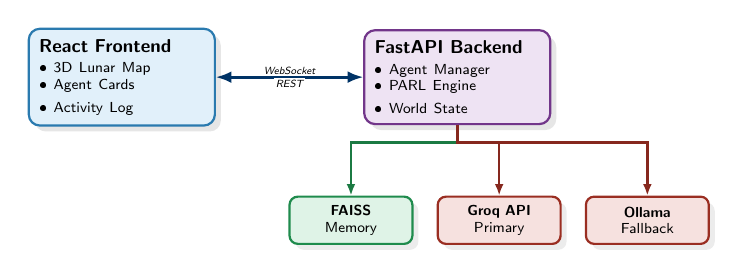
\begin{tikzpicture}[
    scale=0.75, transform shape,
    node distance=1cm and 1.8cm,
    auto,
    mainbox/.style={
        rectangle, draw=#1!80!black, thick, fill=#1!15, 
        text width=2.8cm, inner sep=5pt, align=left, 
        minimum height=1.5cm, rounded corners=4pt, 
        drop shadow={opacity=0.2}, font=\small\sffamily
    },
    servicebox/.style={
        rectangle, draw=#1!80!black, thick, fill=#1!15, 
        text width=1.8cm, inner sep=4pt, align=center, 
        minimum height=0.8cm, rounded corners=3pt, 
        drop shadow={opacity=0.15}, font=\scriptsize\sffamily
    },
    apiflow/.style={draw=isroblue, line width=1pt, {Latex[length=2mm]}-{Latex[length=2mm]}},
    serviceflow/.style={draw=#1!70!black, line width=0.9pt, -{Latex[length=1.5mm]}},
    flowlabel/.style={font=\tiny\sffamily\itshape, fill=white, inner sep=1pt}
]
    \definecolor{frontendblue}{RGB}{52, 152, 219}
    \definecolor{backendviolet}{RGB}{142, 68, 173}
    \definecolor{memorygreen}{RGB}{39, 174, 96}

    \node[mainbox=frontendblue] (frontend) {\textbf{React Frontend}\\[2pt]{\scriptsize • 3D Lunar Map\\ • Agent Cards\\ • Activity Log}};
    \node[mainbox=backendviolet, right=2.5cm of frontend] (backend) {\textbf{FastAPI Backend}\\[2pt]{\scriptsize • Agent Manager\\ • PARL Engine\\ • World State}};
    \node[servicebox=memorygreen, below=1.2cm of backend, xshift=-1.8cm] (faiss) {\textbf{FAISS}\\Memory};
    \node[servicebox=llmred, right=0.4cm of faiss] (groq) {\textbf{Groq API}\\Primary};
    \node[servicebox=llmred, right=0.4cm of groq] (ollama) {\textbf{Ollama}\\Fallback};
    
    \draw[apiflow] (frontend) -- node[flowlabel, above] {WebSocket} node[flowlabel, below] {REST} (backend);
    \draw[serviceflow=memorygreen] (backend.south) -- ++(0,-0.3) -| (faiss.north);
    \draw[serviceflow=llmred] (backend.south) -- ++(0,-0.3) -| (groq.north);
    \draw[serviceflow=llmred] (backend.south) -- ++(0,-0.3) -| (ollama.north);
\end{tikzpicture}
\end{center}

\subsection{Technology Stack}

\begin{table}[H]
\centering
\small
\begin{tabular}{|l|l|}
\hline
\textbf{Layer} & \textbf{Technology} \\
\hline
Frontend & React + Vite + Three.js \\
Backend & Python + FastAPI \\
Real-time & WebSocket \\
Primary LLM & Groq API (llama-3.1-8b-instant) \\
Fallback LLM & Ollama (local) \\
Memory Store & FAISS (vector DB) \\
\hline
\end{tabular}
\end{table}

\subsection{Data Flow}

\begin{enumerate}[leftmargin=*]
    \item \textbf{User Input:} The user starts simulation with parameters
    \item \textbf{Backend:} System initializes agents with their personalities
    \item \textbf{Simulation Loop:} Each agent goes through Perceive, Reason, Act, Learn cycle
    \item \textbf{Frontend:} The UI renders agent positions, activities, and conversations in 3D
    \item \textbf{Logging:} All interactions are stored for later analysis
\end{enumerate}

\subsection{API Endpoints}

\begin{table}[H]
\centering
\small
\begin{tabular}{|l|l|l|}
\hline
\textbf{Endpoint} & \textbf{Method} & \textbf{Purpose} \\
\hline
\texttt{/api/agents/\{name\}/memories} & GET & Retrieve memory stream \\
\texttt{/api/agents/\{name\}/relationships} & GET & Get relationship data \\
\texttt{/api/agents/\{name\}/plan} & GET & Fetch daily schedule \\
\texttt{/api/events/\{id\}/trigger} & POST & Trigger simulation event \\
\texttt{/api/analytics} & GET & Propagation summary \\
\hline
\end{tabular}
\end{table}

%----------------------------------------------------------
\section*{References}
%----------------------------------------------------------
\small
\begin{enumerate}[leftmargin=*]
    \item Park, J.S., et al. (2023). ``Generative Agents: Interactive Simulacra of Human Behavior.'' \textit{arXiv:2304.03442}
    \item Russell, S., \& Norvig, P. (2020). ``Artificial Intelligence: A Modern Approach.'' 4th Edition
    \item ISRO. (2023). ``Chandrayaan-3 Mission Overview.'' Indian Space Research Organisation
\end{enumerate}

\vfill
\begin{center}
\end{center}

\end{document}